
\chapter{Calculs angulaires}

Définitions et notations des formules mathématiques 
et fonctions classiques manipulant les angles et les orientations
utilisées tout au long de ce manuscrit.

\section{Matrices de rotations\label{sec:rotation_matrix}}

La matrice de rotation du plan est notée :
$$
\bm{R}_{\text{2d}}(\theta)
=
\begin{bmatrix}
\mathsf{cos}(\theta) & -\mathsf{sin}(\theta) \\
\mathsf{sin}(\theta) & \mathsf{cos}(\theta) \\
\end{bmatrix}
\in SO(2),~\theta \in \mathbb{R}
$$
Les trois rotations élémentaires de l'espace sont les suivantes :
%Rx
$$
\bm{R}_x(\theta_{\text{roll}})
=
\begin{bmatrix}
1 & 0 & 0 \\
0 & \mathsf{cos}(\theta_{\text{roll}}) & -\mathsf{sin}(\theta_{\text{roll}}) \\
0 & \mathsf{sin}(\theta_{\text{roll}}) & \mathsf{cos}(\theta_{\text{roll}}) \\
\end{bmatrix}
\in SO(3),~\theta_{\text{roll}} \in \mathbb{R}
$$
%Ry
$$
\bm{R}_y(\theta_{\text{pitch}})
=
\begin{bmatrix}
\mathsf{cos}(\theta_{\text{pitch}}) & 0 & \mathsf{sin}(\theta_{\text{pitch}}) \\
0 & 1 & 0 \\
-\mathsf{sin}(\theta_{\text{pitch}}) & 0 & \mathsf{cos}(\theta_{\text{pitch}}) \\
\end{bmatrix}
\in SO(3),~\theta_{\text{pitch}} \in \mathbb{R}
$$
%Rz
$$
\bm{R}_z(\theta_{\text{yaw}})
=
\begin{bmatrix}
\mathsf{cos}(\theta_{\text{yaw}}) & -\mathsf{sin}(\theta_{\text{yaw}}) & 0\\
\mathsf{sin}(\theta_{\text{yaw}}) & \mathsf{cos}(\theta_{\text{yaw}}) & 0\\
0 & 0 & 1 \\
\end{bmatrix}
\in SO(3),~\theta_{\text{yaw}} \in \mathbb{R}
$$

\section{Angles de Cardan\label{sec:angles_euler}}

Les angles de Cardan (ou de Tait-Bryan) sont une manière possible de 
représenter les rotations de l'espace tridimensionnel.
Plus précisément, il s'agit de la composition non commutative
de trois rotations d'angles donnés prises parmi les rotations élémentaires 
de l'espace autour des axes $\vec{\bm{x}}, \vec{\bm{y}}, \vec{\bm{z}}$.
Ils sont également parfois improprement appelés angles d'Euler dans la littérature 
et mais surtout dans les implémentations.
Leur avantage est d'être assez intuitif
et compréhensible par l'humain mais présentent
des configurations singulières où une même orientation
est représentée par une infinité de triplets d'angles.
De plus, la matrice jacobienne est alors non inversible.\\

Parmi les $6$ combinaisons possibles d'angles de Cardan
(et les $6$ combinaisons d'angles d'Euler), 
nous utilisons principalement ici la convention \textit{Z-Y-X} ou \textit{Yaw-Pitch-Roll} 
(Lacet-Tangage-Roulis).
La base flottante (six degrés de liberté) du modèle géométrique 
du robot permet de placer le pied de support à une position
et une orientation donnée dans le monde. 
Le choix de l'ordre de ces degrés de liberté \og virtuels \fg en rotation 
est justement \textit{Yaw-Pitch-Roll}.
Ceci permet une fois le pied sur le sol de fixer l'azimut du robot
en modifiant indépendamment l'angle en lacet sans avoir à recalculer 
les deux autres angles (roulis et tangage) déterminant l'inclinaison 
du pied par rapport au sol.
Les angles de Cardan sont dont définis par le triplet :
$$
(\theta_{\text{yaw}}, \theta_{\text{pitch}}, \theta_{\text{roll}}) 
\in~\big]-\pi,\pi\big] \times \big[-\frac{\pi}{2},\frac{\pi}{2}\big] \times \big]-\pi,\pi\big] \subset \mathbb{R}^3
$$

La fonction suivante est utilisée pour construire la matrice de rotation
$\bm{R}$ à partir du vecteur des angles de Cardan :
$$
\mathsf{CardanToMatrix} :
\begin{bmatrix}
\theta_{\text{roll}} \\
\theta_{\text{pitch}} \\
\theta_{\text{yaw}} \\
\end{bmatrix}
\longmapsto
\bm{R} =
\bm{R}_x(\theta_{\text{roll}}) . \bm{R}_y(\theta_{\text{pitch}}) . \bm{R}_z(\theta_{\text{yaw}})
\in SO(3)
$$

Enfin, la transformation inverse recalcule le vecteur des angles de Cardan associés 
à la matrice de rotation $\bm{R}$ :
$$
\mathsf{MatrixToCardan} : \bm{R} \longmapsto
\begin{bmatrix}
\theta_{\vec{\bm{x}}} \\
\theta_{\vec{\bm{y}}} \\
\theta_{\vec{\bm{z}}} \\
\end{bmatrix}
= 
\begin{bmatrix}
\theta_{\text{roll}} \\
\theta_{\text{pitch}} \\
\theta_{\text{yaw}} \\
\end{bmatrix}
= 
\begin{bmatrix}
\mathsf{atan2}\big(r_{2,1},~r_{2,2}\big) \\
\mathsf{atan2}\big(r_{2,0},~\sqrt{r_{0,0}^2+r_{1,0}^2}\big) \\
\mathsf{atan2}\big(r_{1,0},~r_{0,0}\big) \\
\end{bmatrix}
\in \mathbb{R}^3
$$
où :
$$
\bm{R} = 
\begin{bmatrix}
r_{0,0} & r_{0,1} & r_{0,2} \\
r_{1,0} & r_{1,1} & r_{1,2} \\
r_{2,0} & r_{2,1} & r_{2,2} \\
\end{bmatrix}
\in SO(3)
$$

\section{Distance angulaire\label{sec:distance_angle}}

La distance signée entre les deux angles de $\theta_1$ à $\theta_2$ dans
$]-\pi,\pi]$ se calcule comme suit :
\begin{gather*}
\mathsf{angleDistance} : (\theta_1,\theta_2) \longmapsto\\
d = 
\begin{cases}
    \theta_2-\theta_1 \text{ si }|\theta_2 - \theta_1| < 2\pi - |\theta_2 - \theta_1| \\
    -\mathsf{sign}\big(\theta_2 - \theta_1 \big).\big(2\pi - |\theta_2-\theta_1|\big) \text{ sinon}
\end{cases}
\in ]-\pi,\pi]
\end{gather*}

\section{Normalisation\label{bound_angle}}

La fonction suivante borne un angle dans l'intervalle 
$]-\pi,\pi]$.

$$
\mathsf{angleBound} : \theta \in \mathbb{R} 
\longmapsto \theta - 2\pi\lfloor\frac{\theta + \pi}{2\pi}\rfloor 
$$

\section{Vecteur de rotation\label{sec:axis_angle}}

Les rotations de l'espace peuvent également être représentées
sous une forme appelée \og vecteur de rotation \fg (\textit{axis angle}).
Une rotation peut être caractérisée par un axe de rotation et un angle.
Ici, l'axe et l'angle sont représentés conjointement sous 
la forme d'un vecteur de l'espace. 
Sa direction et son sens donne l'axe de rotation 
et sa norme l'angle de rotation.\\

La conversion d'une matrice de rotation $\bm{R} \in SO(3)$ 
en vecteur de rotation se fait de la manière suivante :
$$
\mathsf{MatrixToAxis} : \bm{R} \longmapsto
\frac{\theta}{||\bm{s}||}.\bm{s} ~\in \mathbb{R}^{3}
$$
avec,
$$
\bm{R} = 
\begin{bmatrix}
r_{0,0} & r_{0,1} & r_{0,2} \\
r_{1,0} & r_{1,1} & r_{1,2} \\
r_{2,0} & r_{2,1} & r_{2,2} \\
\end{bmatrix}
\in SO(3)
$$
$$
\bm{s} = 
\begin{bmatrix}
    r_{2,1} - r_{1,2} \\
    r_{0,2} - r_{2,0} \\
    r_{1,0} - r_{0,1} \\
\end{bmatrix}
\in \mathbb{R}^3
$$
$$
\theta = \mathsf{arcsin}\left(\frac{||\bm{s}||}{2}\right)
\in ]-\frac{\pi}{2},\frac{\pi}{2}]
$$
\newline

L'opération inverse calcul la matrice de rotation à
partir du vecteur de rotation $\bm{a} \in \mathbb{R}^3$ et de la formule de Rodrigues :
$$
\mathsf{AxisToMatrix} : \bm{a} \longmapsto 
\bm{I} + \mathsf{sin}(\theta).\bm{S} + (1-\mathsf{cos}(\theta)).\bm{S}^2 
~\in SO(3)
$$
avec :
$$
\bm{a} = \begin{bmatrix}
    a_x \\
    a_y \\
    a_z \\
\end{bmatrix}
\in \mathbb{R}^3
$$
$$
\theta = ||\bm{a}|| \in \mathbb{R}
$$
$$
\bm{S} = 
\begin{bmatrix}
    0 & -a_z & a_y \\
    a_z & 0 & -a_x \\
    -a_y & a_x & 0 \\
\end{bmatrix}
\in \mathbb{R}^3
$$
\newline

Soit $\bm{a}(t) \in \mathbb{R}^3$ un vecteur de rotation
fonction du temps et représentant l'orientation d'un repère
dans le monde tridimensionnel.
Il est important de noter que la dérivée par rapport au temps 
coefficient par coefficient du vecteur de rotation $\bm{\dot{a}}$ n'est pas 
égale au vecteur de vitesse angulaire $\bm{\omega}$, $\bm{\dot{a}} \neq \bm{\omega}$.
La procédure suivante calcule les vecteurs de vitesse et d'accélération angulaire
corrects à partir du vecteur de rotation et de ces dérivée première et seconde :
$$
\mathsf{AxisDiffToAngularDiff} : \left(\bm{a}, \bm{\dot{a}}, \bm{\ddot{a}}\right) 
\longmapsto \bm{\omega}, \bm{\dot{\omega}} \in \mathbb{R}^3
$$
avec :
\begin{gather*}
\bm{a} = \begin{bmatrix}
    a_x \\
    a_y \\
    a_z \\
\end{bmatrix}
\in \mathbb{R}^3 \\
\theta  = ||\bm{a}|| \in \mathbb{R} \\
c = \mathsf{cos}\left(\frac{\theta}{2}\right) \in \mathbb{R} \\
s = \mathsf{sin}\left(\frac{\theta}{2}\right) \in \mathbb{R} \\
b = \theta c - 2s \in \mathbb{R} \\
W = \frac{1}{\theta}
\begin{bmatrix}
    -a_xs & \theta c & -a_zs & a_ys \\
    -a_ys & a_zs & \theta c & -a_xs \\
    -a_zs & -a_ys & a_xs & \theta c \\
\end{bmatrix}
\in \mathbb{R}^{3 \times 4} \\
G = \frac{1}{2\theta^3}
\begin{bmatrix}
    -a_x\theta^2s & -a_y\theta^2s & -a_z\theta^2s \\
    2\theta^2s + a_x^2b & a_xa_yb & a_xa_zb \\
    a_xa_yb & 2\theta^2s + a_y^2b & a_ya_zb \\
    a_xa_zb & a_ya_zb & 2\theta^2s + a_z^2b \\
\end{bmatrix}
\in \mathbb{R}^{4 \times 3} \\
\bm{\omega} = 
\begin{cases}
    \bm{\dot{a}} \text{ if }\theta=0\\
    2WG\bm{\dot{a}} \text{ else}\\
\end{cases}
\bm{\dot{\omega}} = 
\begin{cases}
    \bm{\ddot{a}}  \text{ if }\theta=0 \\
    2WG\bm{\ddot{a}}  \text{ else}\\
\end{cases}
\end{gather*}

\chapter{Complément à la calibration de l'odométrie proprioceptive 
par optimisation CMA-ES\label{sec:odometry_cmaes_read_plots}}

\begin{figure}[h]
    \centerfloat
    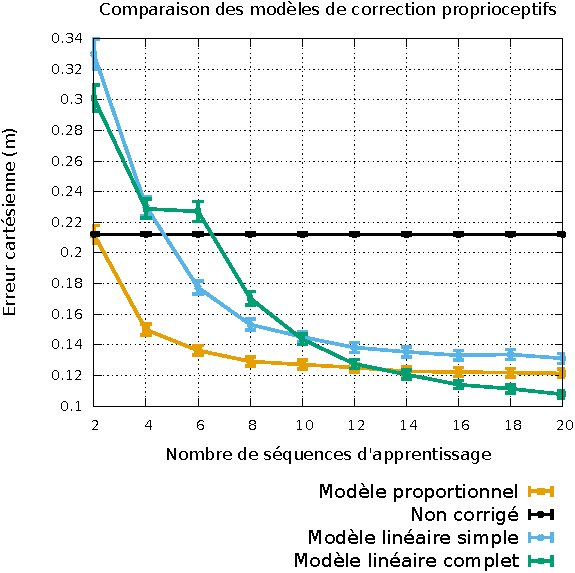
\includegraphics[type=pdf,ext=.pdf,read=.pdf,width=0.8\linewidth]{../plot/OdometryCMAES/convergenceReads}
    \caption{\label{fig:odometry_cmaes_convergence_reads} 
        Convergence et comparaison de l'erreur cartésienne moyenne en position (proprioceptive)
        en fonction du nombre d'enregistrements utilisés pour l'apprentissage.
        Les trois modèles linéaires de corrections sont comparés à l'estimation
        de l'odométrie sans correction.
        Les marges de confiance à $95\%$ sont représentées.
    }
\end{figure}

\begin{figure}[h]
    \centerfloat
    \begin{subfigure}{0.4\paperwidth}
        \centering
        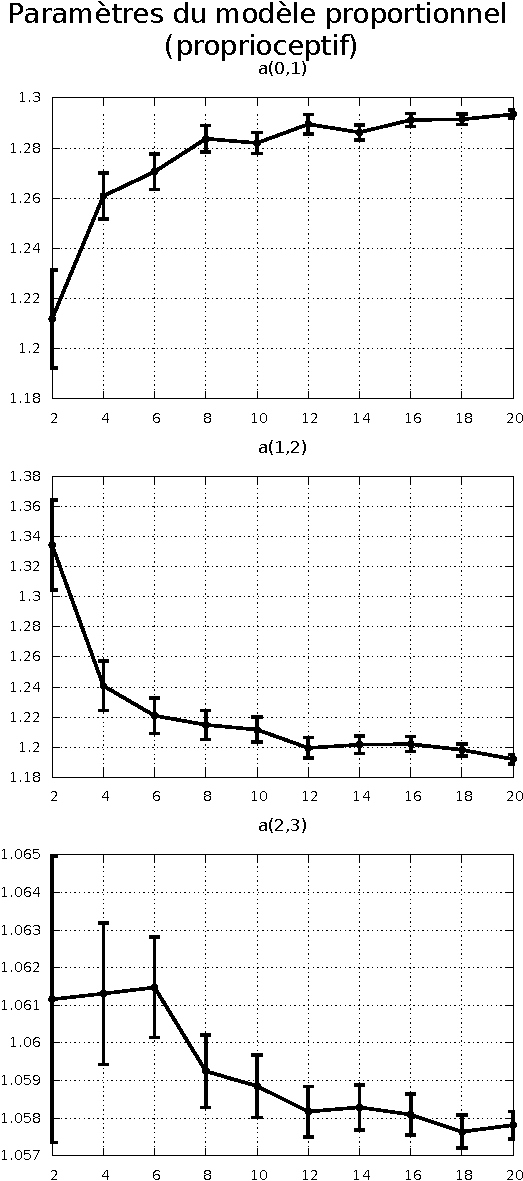
\includegraphics[type=pdf,ext=.pdf,read=.pdf,width=0.7\linewidth]{../plot/OdometryCMAES/parametersPropReads}
    \end{subfigure}
    \begin{subfigure}{0.4\paperwidth}
        \centering
        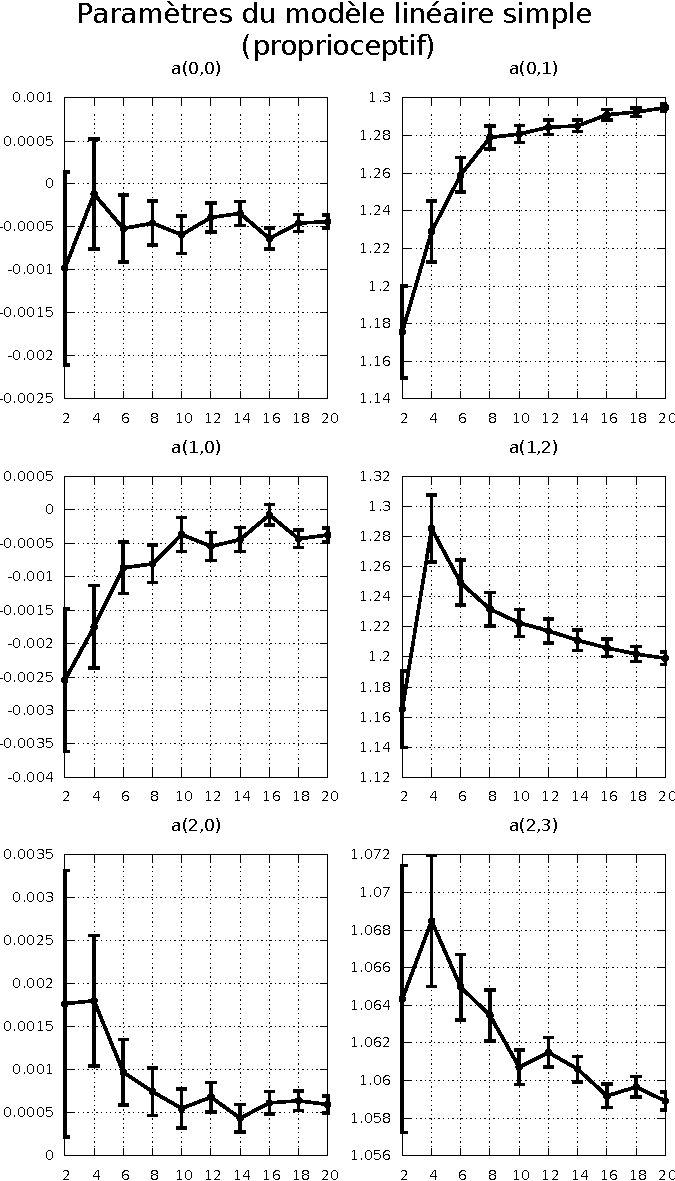
\includegraphics[type=pdf,ext=.pdf,read=.pdf,width=0.9\linewidth]{../plot/OdometryCMAES/parametersSimpleReads}
    \end{subfigure}
    \caption{\label{fig:odometry_cmaes_parameters_prop_simple_reads} 
        Convergence des valeurs moyennes des $3$ et $6$ paramètres des modèles proportionnel 
        et linéaire simple (proprioceptifs) en fonction du nombre de séquences utilisées pour l'apprentissage.
        Les marges de confiance à $95\%$ sont représentées.
    }
\end{figure}
\begin{figure}[h]
    \centerfloat
    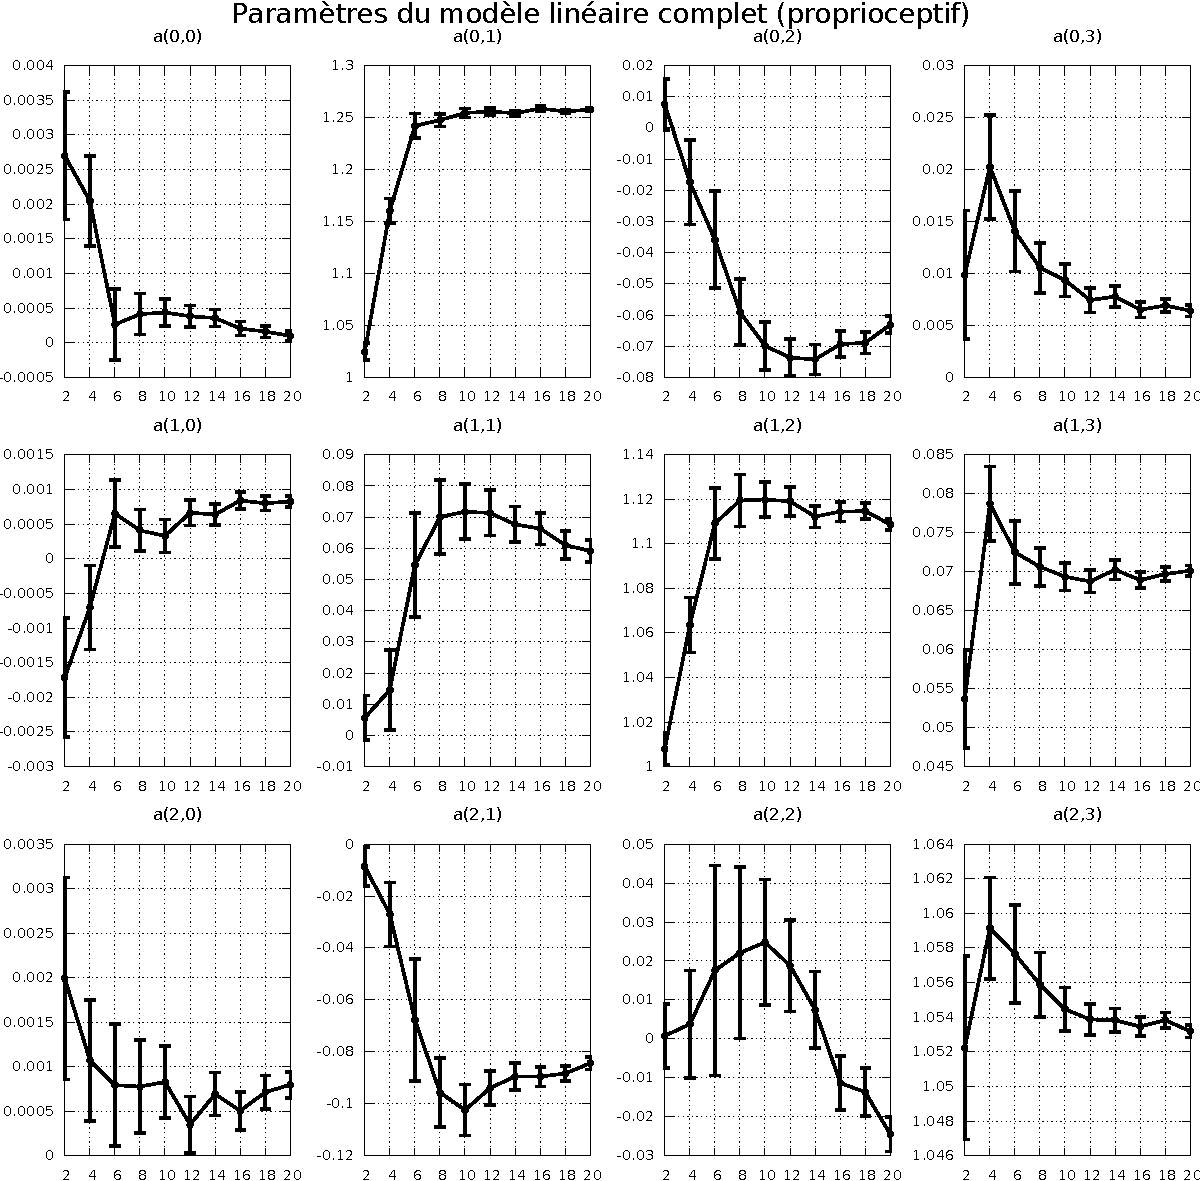
\includegraphics[type=pdf,ext=.pdf,read=.pdf,width=0.9\linewidth]{../plot/OdometryCMAES/parametersFullReads}
    \caption{\label{fig:odometry_cmaes_parameters_full_reads} 
        Convergence des valeurs moyennes des $12$ paramètres du modèle linéaire complet (proprioceptif)
        en fonction du nombre de séquences utilisées pour l'apprentissage.
        Les marges de confiance à $95\%$ sont représentées.
    }
\end{figure}

\begin{figure}[h]
    \centerfloat
    \begin{subfigure}{0.28\paperwidth}
        \centering
        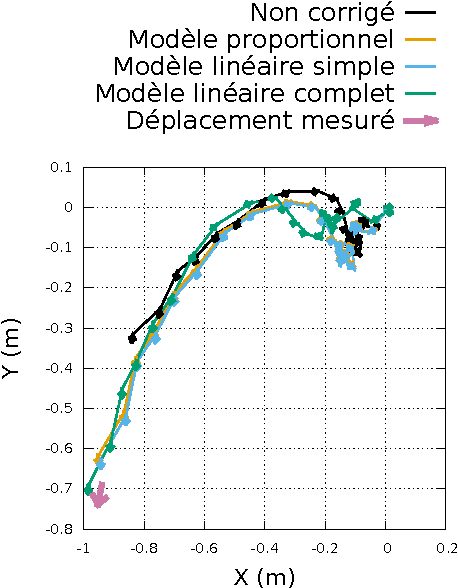
\includegraphics[type=pdf,ext=.pdf,read=.pdf,width=1.0\linewidth]{../plot/OdometryCMAES/readsTraj1}
    \end{subfigure}
    \begin{subfigure}{0.28\paperwidth}
        \centering
        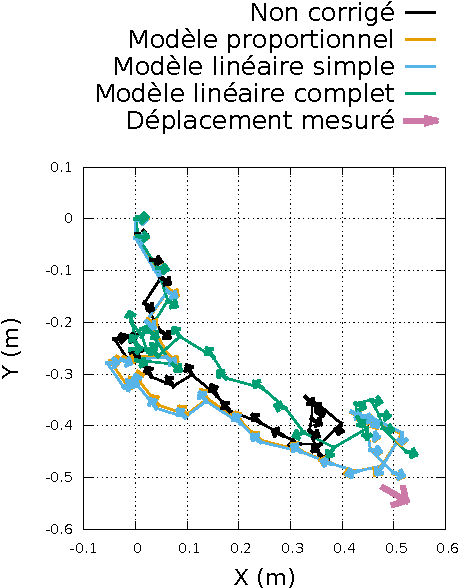
\includegraphics[type=pdf,ext=.pdf,read=.pdf,width=1.0\linewidth]{../plot/OdometryCMAES/readsTraj2}
    \end{subfigure}
    \begin{subfigure}{0.28\paperwidth}
        \centering
        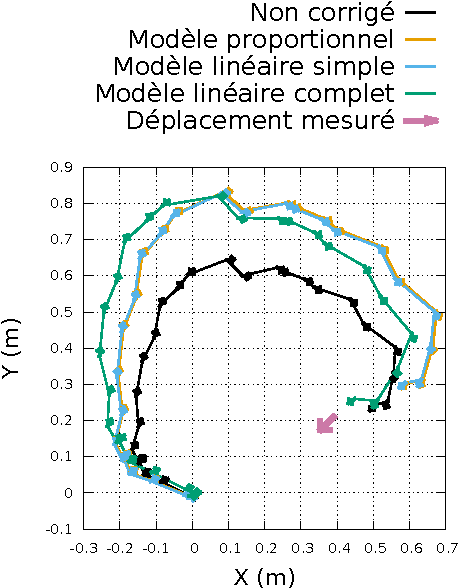
\includegraphics[type=pdf,ext=.pdf,read=.pdf,width=1.0\linewidth]{../plot/OdometryCMAES/readsTraj3}
    \end{subfigure}
    \newline
    \begin{subfigure}{0.28\paperwidth}
        \centering
        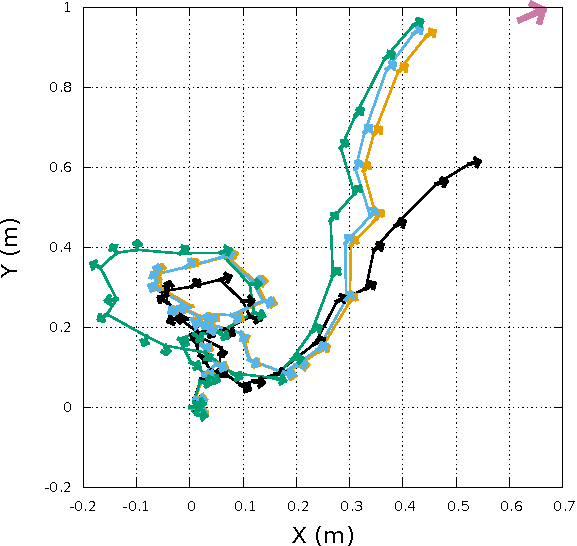
\includegraphics[type=pdf,ext=.pdf,read=.pdf,width=1.0\linewidth]{../plot/OdometryCMAES/readsTraj4}
    \end{subfigure}
    \begin{subfigure}{0.28\paperwidth}
        \centering
        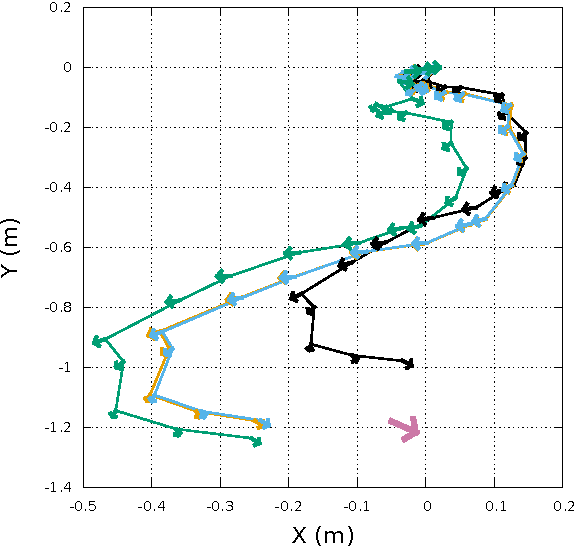
\includegraphics[type=pdf,ext=.pdf,read=.pdf,width=1.0\linewidth]{../plot/OdometryCMAES/readsTraj5}
    \end{subfigure}
    \begin{subfigure}{0.28\paperwidth}
        \centering
        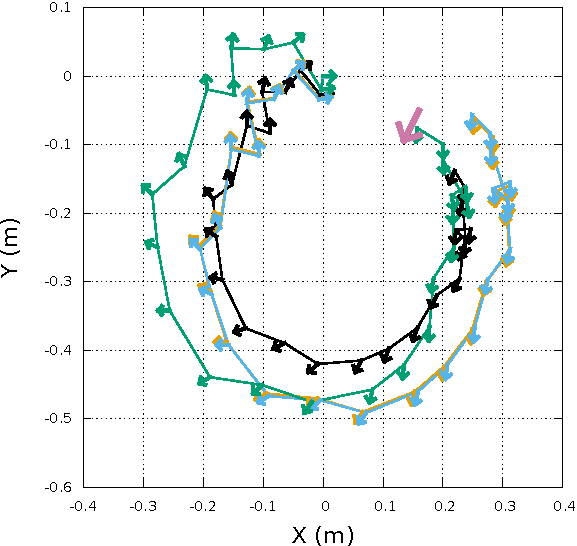
\includegraphics[type=pdf,ext=.pdf,read=.pdf,width=1.0\linewidth]{../plot/OdometryCMAES/readsTraj6}
    \end{subfigure}
    \newline
    \begin{subfigure}{0.28\paperwidth}
        \centering
        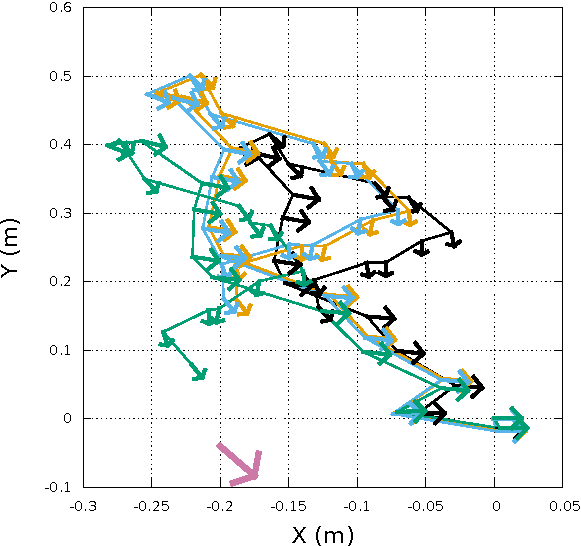
\includegraphics[type=pdf,ext=.pdf,read=.pdf,width=1.0\linewidth]{../plot/OdometryCMAES/readsTraj7}
    \end{subfigure}
    \begin{subfigure}{0.28\paperwidth}
        \centering
        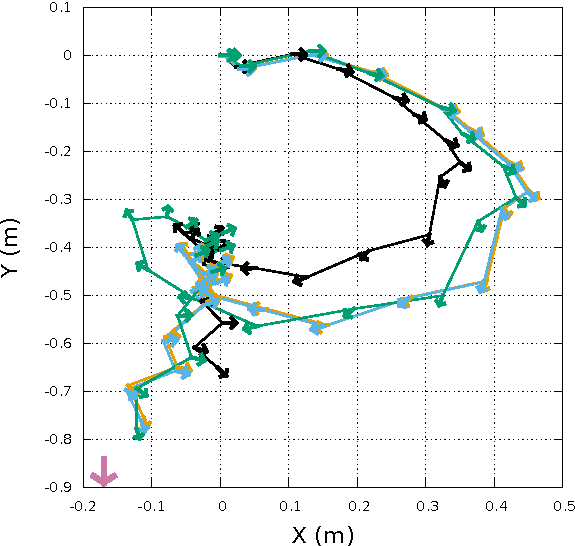
\includegraphics[type=pdf,ext=.pdf,read=.pdf,width=1.0\linewidth]{../plot/OdometryCMAES/readsTraj8}
    \end{subfigure}
    \begin{subfigure}{0.28\paperwidth}
        \centering
        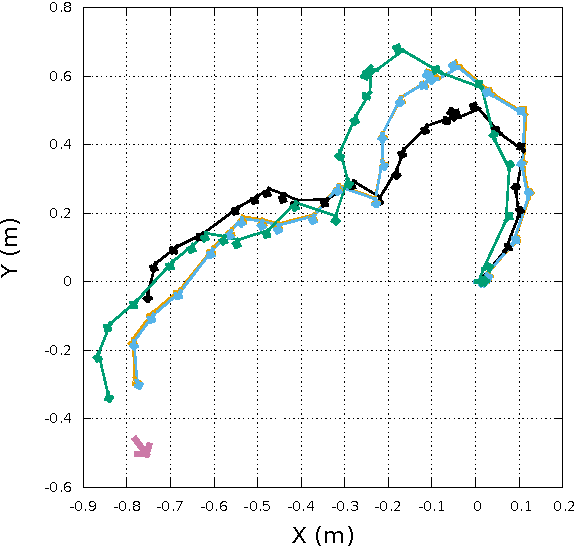
\includegraphics[type=pdf,ext=.pdf,read=.pdf,width=1.0\linewidth]{../plot/OdometryCMAES/readsTraj9}
    \end{subfigure}
    \caption{\label{fig:odometry_cmaes_trajs_reads} 
        Comparaison sur neuf des séquences enregistrées de l'odométrie proprioceptive non
        corrigée et corrigée par les trois modèles linéaires après calibration.
        La pose finale mesurée est également représentée.
        Chaque point le long des trajectoires correspond à la pose estimée du robot 
        au début de chaque cycle de marche.
        La pose de départ est centrée sur zéro.
    }
\end{figure}

